\documentclass[margin=10pt]{standalone}
\usepackage{color,xcolor}
\usepackage{makecell}
\usepackage{tikz-qtree, tikz}
\usetikzlibrary{arrows.meta,bending}
\usetikzlibrary{calc,trees,positioning,arrows,chains,shapes, shapes.geometric,%
    decorations.pathreplacing,decorations.pathmorphing,decorations.markings,shapes,%
    matrix,shapes.symbols,positioning,angles,quotes,patterns}
\usepackage[utf8]{inputenc}

\def\centerarc[#1](#2)(#3:#4:#5)% Syntax: [draw options] (center) (initial angle:final angle:radius)
    { \draw[#1] ($(#2)+({#5*cos(#3)},{#5*sin(#3)})$) arc (#3:#4:#5); }

%See https://tex.stackexchange.com/a/29367/1952
\makeatletter
\tikzset{% customization of pattern
        hatch distance/.store in=\hatchdistance,
        hatch distance=5pt,
        hatch thickness/.store in=\hatchthickness,
        hatch thickness=5pt
        }
\pgfdeclarepatternformonly[\hatchdistance,\hatchthickness]{north east hatch}% name
    {\pgfqpoint{-1pt}{-1pt}}% below left
    {\pgfqpoint{\hatchdistance}{\hatchdistance}}% above right
    {\pgfpoint{\hatchdistance-1pt}{\hatchdistance-1pt}}%
    {
        \pgfsetcolor{\tikz@pattern@color}
        \pgfsetlinewidth{\hatchthickness}
        \pgfpathmoveto{\pgfqpoint{0pt}{0pt}}
        \pgfpathlineto{\pgfqpoint{\hatchdistance}{\hatchdistance}}
        \pgfusepath{stroke}
    }
\makeatother

% Drawing spirals
\makeatletter
\newif\ifspiral@is@clockwise
  \pgfkeys{
    spiral/.is family,
    spiral,
    start angle/.initial=0,
    end angle/.initial=0,
    start radius/.initial=0,
    end radius/.initial=1,
    revolutions/.initial=2,
    name/.initial=,
    center/.initial={(0,0)},
    sample rate/.initial =5,
    clockwise spiral/.is if=spiral@is@clockwise,
    clockwise spiral/.default=false,
    clockwise/.style={clockwise spiral=true},
    default spiral/.style={start angle=0,end angle=0, start radius=0, end radius=1, revolutions=2, name=, center={(0,0)}, sample rate=5, clockwise spiral=false}
  }
  \newcommand\spiral[2][]{
    \pgfkeys{spiral, default spiral,#2,
      start angle/.get=\spiral@start@angle,
      end angle/.get=\spiral@end@angle,
      start radius/.get=\spiral@start@radius,
      end radius/.get=\spiral@end@radius,
      revolutions/.get=\spiral@revolutions,
      name/.get=\spiral@name,
      sample rate/.get=\spiral@sample@rate,
      center/.get=\spiral@center
      }
  \def\spiral@start@name{}
  \def\spiral@end@name{}
  \ifspiral@is@clockwise
        \renewcommand*{\spiral@start@angle}{\pgfkeysvalueof{/spiral/end angle}}
        \renewcommand*{\spiral@end@angle}{\pgfkeysvalueof{/spiral/start angle}}
        \renewcommand*{\spiral@start@radius}{\pgfkeysvalueof{/spiral/end radius}}
        \renewcommand*{\spiral@end@radius}{\pgfkeysvalueof{/spiral/start radius}}
        \if\relax\detokenize{\spiral@name}\relax
        \else
          \renewcommand*{\spiral@start@name}{\spiral@name end}
          \renewcommand*{\spiral@end@name}{\spiral@name start}
        \fi
    \else
        \if\relax\detokenize{\spiral@name}\relax
        \else
          \renewcommand*{\spiral@start@name}{\spiral@name start}
          \renewcommand*{\spiral@end@name}{\spiral@name end}
        \fi
  \fi
  \pgfmathsetmacro{\spiral@domain}{\spiral@end@angle+\spiral@revolutions*360}
  \pgfmathsetmacro{\spiral@growth}{180*(\spiral@end@radius-\spiral@start@radius)/(pi*(\spiral@domain-\spiral@start@angle))}
  \draw [#1,
         shift={\spiral@center},
         domain=\spiral@start@angle*pi/180:\spiral@domain*pi/180,
         variable=\t,
         smooth,
         samples=int(\spiral@domain/\spiral@sample@rate)] node[coordinate,shift={(\spiral@start@angle:\spiral@start@radius)}](\spiral@start@name){} plot ({\t r}: {\spiral@start@radius+\spiral@growth*\t-\spiral@growth*\spiral@start@angle*pi/180}) node[coordinate](\spiral@end@name){}
  }
\makeatother

\definecolor{myblue}{HTML}{0072BD}
\definecolor{mygreen}{HTML}{258F1B}
\definecolor{myred}{HTML}{C4000C}

\newcommand{\Ms}{\ensuremath{M_\mathrm{s}}} % Martensite start Temperature
\newcommand{\Mf}{\ensuremath{M_\mathrm{f}}} % Martensite finish Temperature
\newcommand{\As}{\ensuremath{A_\mathrm{s}}} % Austenite start Temperature
\newcommand{\Af}{\ensuremath{A_\mathrm{f}}} % Austenite finish Temperature

\tikzset{
  pivot_node/.style = {
    inner sep=0pt, minimum width=1.67cm,minimum height=0.75cm,
    path picture={
    % screen (with border)
        \node (piv) {};
        \spiral[thick]{start radius=0.01, end radius=0.25, revolutions=3, center={(piv.center)}, clockwise, name=clockwisespiral};
        \draw [black,thick,domain=25:335] plot ({0.35*cos(\x)}, {0.35*sin(\x)});
        \draw[thick] ($(piv.center)+({0.35*cos(25)},{0.35*sin(25)})$) -- +(0.5cm,0) node (end1){};
        \draw[thick] ($(piv.center)+({0.35*cos(25)},{-0.35*sin(25)})$) -- +(0.5cm,0) node (end2){};
        \draw[thick] (end1.center) -- (end2.center);
    }
  }
}


\begin{document}
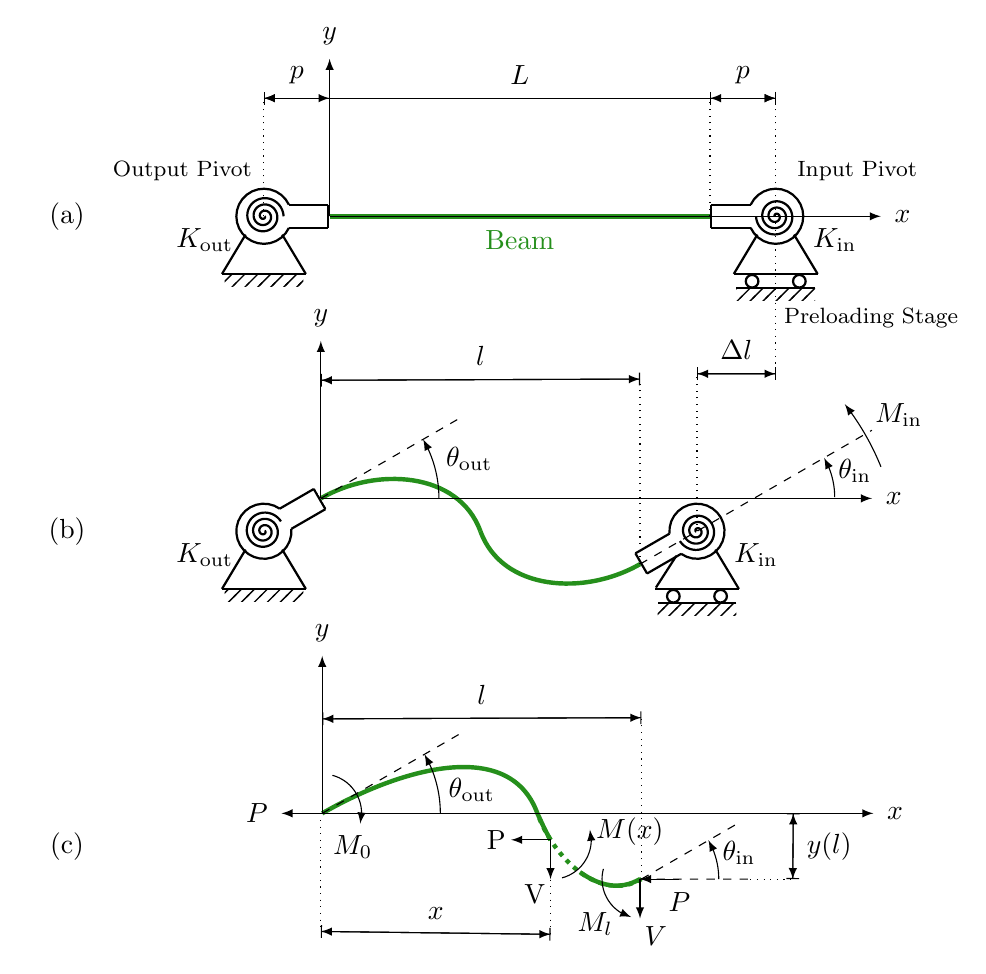
\begin{tikzpicture}[every node/.style={inner sep=0,outer sep=0}]
\tikzstyle{sma}=[ultra thick,decorate,decoration={zigzag,pre length=4mm,post length=4mm,segment length=5mm, amplitude=2.5mm}]
\tikzstyle{spring}=[ultra thick,decoration={aspect=0.5,pre length=4mm,post length=4mm,segment length=4mm, amplitude=2.5mm,coil},decorate]
\tikzstyle{ground}=[pattern=north east hatch, hatch distance=2mm, hatch thickness=.5pt, fill,draw=none,minimum width=2mm,minimum height=0.1mm]

\tikzstyle{smalong}=[ultra thick,decorate,decoration={zigzag,pre length=4mm,post length=4mm,segment length=9mm, amplitude=2.5mm}]
\tikzstyle{springshort}=[ultra thick,decoration={aspect=0.5,pre length=4mm,post length=4mm,segment length=2mm, amplitude=2.5mm,coil},decorate]

\tikzstyle{smarest}=[ultra thick,decorate,decoration={zigzag,pre length=4mm,post length=4mm,segment length=3.5mm, amplitude=2.5mm}]
\tikzstyle{springrest}=[ultra thick,decoration={aspect=0.5,pre length=4mm,post length=4mm,segment length=1.5mm, amplitude=2.5mm,coil},decorate]

    % SMA - Spring (Hot)
    \node[pivot_node] (M1) at (0,0) {}; % Pivot left
        % <Triangle>
        \draw [thick] ($(M1.center)+({-0.55*sin(25)},{-0.55*sin(25)})$) -- +(-0.3,-0.5) node (end1){};
        \draw [thick] ($(M1.center)+({0.55*sin(25)},{-0.55*sin(25)})$) -- +(0.3,-0.5) node (end2){};
        \draw[thick] (end1.center) -- (end2.center); % <\Triangle>
        \node (ground1) [ground,anchor=north,minimum width=1cm,minimum height=0.15cm, yshift=-21] at (M1.center) {}; % Ground hatch
    \node[pivot_node, rotate=180] (M2) at ($(M1.center)+(6.5,0)$) {};   % Pivot right
        % <Triangle
        \draw [thick] ($(M2.center)+({-0.55*sin(25)},{-0.55*sin(25)})$) -- +(-0.3,-0.5) node (end1){};
        \draw [thick] ($(M2.center)+({0.55*sin(25)},{-0.55*sin(25)})$) -- +(0.3,-0.5) node (end2){};
        \draw[thick] (end1.center) -- (end2.center); % <\Triangle>
        \node (ground2) [ground,anchor=north,minimum width=1cm,minimum height=0.15cm, yshift=-26] at (M2.center) {}; % Gound hatch
        \draw[thick] (ground2.north east) -- (ground2.north west); % Ground line
        \draw[draw,thick,anchor=north] ($(M2.south)+(0.3,-1.2)$) circle (0.08); % Wheel
        \draw[draw,thick,anchor=south] ($(M2.south)+(-0.3,-1.2)$) circle (0.08); % Wheel
    \draw [ultra thick, color=mygreen] (M1.east) -- node[pos=0.5, below, outer sep=5] {Beam }(M2.east); % Beam
    % <Axis>
    \draw[-latex, thin] (M1.east) -- +(7,0) node[right, outer sep=5] {$x$};
    \draw[-latex, thin] (M1.east) -- +(0,2) node[above, outer sep=5] {$y$}; % <\Axis>
    % <L Label>
    \node[yshift=+1.5cm, draw=none] (xc) at (M1.center) {};
    \node[yshift=+1.5cm, draw=none] (xh) at (M2.center) {};
    \draw[|-|] (xc.center)-- node[above, draw=none, outer sep=5] {$L$} (xh.center);
    \draw[latex-latex] (xc.center)-- (xh.center);
    \draw[dotted] (M1.center)--(xc.center);
    \draw[dotted] (M2.center)--(xh.center);% <\L Label>
    % <p right Label>
    \node[yshift=+1.5cm, draw=none] (xc) at (M1.center) {};
    \node[yshift=+1.5cm, draw=none] (xh) at (M1.east) {};
    \draw[|-|] (xc.center)-- node[above, draw=none, outer sep=5] {$p$} (xh.center);
    \draw[latex-latex] (xc.center)-- (xh.center);
    \draw[dotted] (M1.center)--(xc.center);
    \draw[dotted] (M1.east)--(xh.center);% <\p right Label>
    % <p left Label>
    \node[yshift=+1.5cm, draw=none] (xc) at (M2.center) {};
    \node[yshift=+1.5cm, draw=none] (xh) at (M2.east) {};
    \draw[|-|] (xc.center)-- node[above, draw=none, outer sep=5] {$p$} (xh.center);
    \draw[latex-latex] (xc.center)-- (xh.center);
    \draw[dotted] (M2.center)--(xc.center);
    \draw[dotted] (M2.east)--(xh.center);% <\p left Label>
    % <Labels>
    \node at ($(M1.north west) +(-0.2,0.2)$){\footnotesize Output Pivot};
    \node at ($(M2.south west) +(0.2,0.2)$){\footnotesize Input Pivot};
    \node[align=center, outer sep=3, anchor=north west] at ($(ground2.south) +(0,0)$){\footnotesize Preloading Stage};
    \node[text width=1cm,align=center, outer sep=5] at ($(M2.center) +(0.75,-0.3)$){$K_\mathrm{in}$};
    \node[text width=1cm,align=center, outer sep=5] at ($(M1.center) +(-0.75,-0.3)$){$K_\mathrm{out}$};% <\Labels>
    \node[text width=1cm,align=center, outer sep=5] at ($(M1.center) +(-2.5,0)$){(a)}; % Subfigure label

    %%%%%%%%%%%%%%%%%%%% BUCKLED FIGURE %%%%%%%%%%%%%%%%%%%%%

    \node[pivot_node,rotate=30] (N1) at (0,-4) {}; % Pivot left
        % <Triangle>
        \draw [thick] ($(N1.center)+({-0.55*sin(25)},{-0.55*sin(25)})$) -- +(-0.3,-0.5) node (end1){};
        \draw [thick] ($(N1.center)+({0.55*sin(25)},{-0.55*sin(25)})$) -- +(0.3,-0.5) node (end2){};
        \draw[thick] (end1.center) -- (end2.center); % <\Triangle>
        \node (ground1) [ground,anchor=north,minimum width=1cm,minimum height=0.15cm, yshift=-21] at (N1.center) {}; % Ground hatch
    \node[pivot_node, rotate=210] (N2) at ($(N1.center)+(5.5,0)$) {};   % Pivot right
        % <Triangle
        \node (trirightN2) at ($(N2.center)+({-0.55*sin(25)},{-0.55*sin(25)})$) {};
        \node (trirightN2_end) at ($(trirightN2.center)+(-0.3,-0.5)$) {};
        \draw[thick] ($(N2.center)+({-0.62*sin(25)},{-0.74*sin(25)})$) -- (trirightN2_end) node (end1){};
        \draw [thick] ($(N2.center)+({0.55*sin(25)},{-0.55*sin(25)})$) -- +(0.3,-0.5) node (end2){};
        \draw[thick] (end1.center) -- (end2.center); % <\Triangle>
        \node (ground2) [ground,anchor=north,minimum width=1cm,minimum height=0.15cm, yshift=-26] at (N2.center) {}; % Gound hatch
        \draw[thick] (ground2.north east) -- (ground2.north west); % Ground line
        \draw[draw,thick,anchor=north] ($(N2.center)+(0.3,-0.825)$) circle (0.08); % Wheel
        \draw[draw,thick,anchor=north] ($(N2.center)+(-0.3,-0.825)$) circle (0.08); % Wheel
    \draw [ultra thick, color=mygreen] (N1.east) to[out=30,in=110] ($(N1.center)+(2.75,0)$); % First half beam
    \draw [ultra thick, color=mygreen] (N2.east) to[out=-150,in=-70] ($(N1.center)+(2.75,0)$); % Second half beam
    % <Axis>
    \draw[-latex, thin] (N1.east) -- +(7,0) node[right, outer sep=5] {$x$};
    \draw[-latex, thin] (N1.east) -- +(0,2) node[above, outer sep=5] {$y$}; % <\Axis>
    % <l Label>
    \node[yshift=+1.5cm, draw=none] (xc) at (N1.east) {};
    \node[yshift=+2.35cm, draw=none] (xh) at (N2.east) {};
    \draw[|-|] (xc.center)-- node[above, draw=none, outer sep=5] {$l$} (xh.center);
    \draw[latex-latex] (xc.center)-- (xh.center);
    \draw[dotted] (N1.east)--(xc.center);
    \draw[dotted] (N2.east)--(xh.center);% <\l Label>
    % <deltal right Label>
    \node[yshift=-2cm, draw=none] (xc) at (M2.center) {};
    \node[yshift=+2cm, draw=none] (xh) at (N2.center) {};
    \draw[|-|] (xc.center)-- node[above, draw=none, outer sep=5] {$\Delta l$} (xh.center);
    \draw[latex-latex] (xc.center)-- (xh.center);
    \draw[dotted] (M2.center)--(xc.center);
    \draw[dotted] (N2.center)--(xh.center);% <\deltal right Label>
    % <M in>
    \draw ($(N2.east) +({3.4*cos(38)}, {3.4*sin(38)})$) coordinate (c)
        ($(N2.east) +({3.4*cos(22)}, {3.4*sin(22)})$) coordinate (a)
        (N2.east)coordinate (b)
        pic["$M_\mathrm{in}$",draw, solid,-latex,angle eccentricity=1.15,angle radius=3.3cm] {angle=a--b--c}; % <\M in>
    % <theta in>
    \draw[dashed] (N2.east) -- +({3.4*cos(30)}, {3.4*sin(30)}) coordinate (c)
        ($(N2.east)+({1.7*cos(30)}, {1.7*sin(30)})$)coordinate (b)
        ($(b)+(0.5,0)$) coordinate (a)
        pic["$\theta_\mathrm{in}$",draw, solid,-latex,angle eccentricity=1.3,angle radius=1cm] {angle=a--b--c}; % <\theta in>
    % <theta out>
    \draw[dashed] (N1.east) coordinate (b) -- +({2*cos(30)}, {2*sin(30)}) coordinate (a)
    ($(N1.east)+(1.8,0)$) coordinate (c)
    pic["$\theta_\mathrm{out}$",draw, solid,-latex,angle eccentricity=1.3,angle radius=1.5cm] {angle=c--b--a}; % <\theta out>
    % <Labels>
    \node[text width=1cm,align=center, outer sep=5] at ($(N2.center) +(0.75,-0.3)$){$K_\mathrm{in}$};
    \node[text width=1cm,align=center, outer sep=5] at ($(N1.center) +(-0.75,-0.3)$){$K_\mathrm{out}$};% <\Labels>
    \node[text width=1cm,align=center, outer sep=5] at ($(N1.center) +(-2.5,0)$){(b)}; % Subfigure label

    %%%%%%%%%%%%%%%%%%%% BUCKLED LINE FIGURE %%%%%%%%%%%%%%%%%%%%%

    \node (O1) at ($(N1.east)+(0,-4cm)$) {}; % Pivot left
    \node (O2) at ($(N2.east)+(0,-4cm)$) {}; % Pivot left
    \draw [ultra thick, color=mygreen] (O1.east) to[out=30,in=110] ($(O1.center)+(2.75,0)$) coordinate (P); % First half beam
    \draw [ultra thick, color=mygreen, dotted] (O2.east) to[out=-150,in=-70] node[pos=0.5] (P1) {} node[pos=0.8] (P2) {} node[pos=0.9] (Pend) {} ($(O1.center)+(2.75,0)$); % Second half beam
        \draw [ultra thick, color=mygreen] (P.center) to[out=-65,in=120] (P2.center); % First half solid line
        \draw [ultra thick, color=mygreen] (P1.center) to[out=-35,in=-150] (O2.center); % Second half solid line
        \draw[-latex] (P2.center) -- +(0,-0.5) node[below, outer sep=2, xshift=-0.2cm] {V};
        \draw[-latex] (P2.center) -- +(-0.5,0) node[left, outer sep=2] {P};
    % <Axis>
    \draw[-latex, thin] (O1.east) -- +(7,0) node[right, outer sep=5] {$x$};
    \draw[-latex, thin] (O1.east) -- +(0,2) node[above, outer sep=5] {$y$}; % <\Axis>
    \draw[latex-, thin] ($(O1.center)+(-0.5,0)$) node[left, outer sep=5] {$P$} -- (O1.center) ; % P load arrow
    \draw[-latex, thin] ($(O2.center)+(0.5,0)$) node[below, outer sep=5] {$P$} -- (O2.center) ; % P load arrow right
    \draw[latex-, thin] ($(O2.center)+(0,-0.5)$) node[below, outer sep=3, xshift=0.2cm] {$V$} -- (O2.center) ; % V load arrow right
    % <l Label>
    \node[yshift=+1.2cm, draw=none] (xc) at (O1.east) {};
    \node[yshift=+2.05cm, draw=none] (xh) at (O2.east) {};
    \draw[|-|] (xc.center)-- node[above, draw=none, outer sep=5] {$l$} (xh.center);
    \draw[latex-latex] (xc.center)-- (xh.center);
    \draw[dotted] (O1.east)--(xc.center);
    \draw[dotted] (O2.east)--(xh.center);% <\l Label>
    % <x Label>
    \node[yshift=-1.5cm, draw=none] (xc) at (O1.center) {};
    \node[yshift=-1.2cm, draw=none] (xh) at (P2.center) {};
    \draw[|-|] (xc.center)-- node[above, draw=none, outer sep=5] {$x$} (xh.center);
    \draw[latex-latex] (xc.center)-- (xh.center);
    \draw[dotted] (O1.center)--(xc.center);
    \draw[dotted] (P2.center)--(xh.center);% <\x Label>
    % <M0 in>
    \draw ($(O1.east) +({0.4*cos(75)}, {0.4*sin(75)})$) coordinate (m0c)
        ($(O1.east) +({0.4*cos(-15)}, {0.4*sin(-15)})$) coordinate (m0a) node[below, outer sep=5] {$M_0$}
        (O1.east)coordinate (m0b)
        pic["",draw, solid,latex-,angle eccentricity=0.15,angle radius=0.5cm] {angle=m0a--m0b--m0c}; % <\M0 in>
    % <Ml in>
    \draw ($(O2.east) +({-0.4*cos(75)}, {-0.4*sin(75)})$) coordinate (m0c)
        ($(O2.east) +({-0.4*cos(-15)}, {-0.4*sin(-15)})$) coordinate (m0a) node[above, outer sep=5,yshift=-1cm, xshift=-0.2cm] {$M_l$}
        (O2.east)coordinate (m0b)
        pic["",draw, solid,-latex,angle eccentricity=0.15,angle radius=0.5cm] {angle=m0a--m0b--m0c}; % <\Ml in>
    % <Mx in>
    \draw ($(P2.east) +({0.4*cos(75)}, {-0.4*sin(75)})$) coordinate (m0c)
        ($(P2.east) +({0.4*cos(-15)}, {-0.4*sin(-15)})$) coordinate (m0a) node[right, outer sep=5, xshift=0cm] {$M(x)$}
        (P2.east)coordinate (m0b)
        pic["",draw, solid,-latex,angle eccentricity=0.15,angle radius=0.5cm] {angle=m0c--m0b--m0a}; % <\Mx in>
    % <theta in>
    \draw[dashed] (O2.east) -- +({1.4*cos(30)}, {1.4*sin(30)}) coordinate (cti)
        (O2.center) coordinate (bti)
        -- ($(bti)+(1.4,0)$) coordinate (ati)
        pic["$\theta_\mathrm{in}$",draw, solid,-latex,angle eccentricity=1.3,angle radius=1cm] {angle=ati--bti--cti}; % <\theta in>
    % <theta out>
    \draw[dashed] (O1.east) coordinate (bto) -- +({2*cos(30)}, {2*sin(30)}) coordinate (ato)
    ($(O1.east)+(1.8,0)$) coordinate (cto) node[xshift=0.1cm, yshift=0.3cm] {$\theta_\mathrm{out}$}
    pic["",draw, solid,-latex,angle eccentricity=1.3,angle radius=1.5cm] {angle=cto--bto--ato}; % <\theta out>
    % <y(l) Label>
    \node[xshift=0.54cm, draw=none] (xc) at (ati.center) {};
    \node[xshift=6cm, draw=none] (xh) at (O1.center) {};
    \draw[|-|] (xc.center)-- node[right, draw=none, outer sep=5] {$y(l)$} (xh.center);
    \draw[latex-latex] (xc.center)-- (xh.center);
    \draw[dotted] (ati.center)--(xc.center);
    \draw[dotted] (O1.center)--(xh.center);% <\y(l) Label>
    \node[text width=1cm,align=center, outer sep=5] at ($(N1.center) +(-2.5,-4)$){(c)}; % Subfigure label
\end{tikzpicture}
\end{document}
